\subsection{Massive Static Yukawa Results}
\label{sec:static_yukawa}

Before looking at results for the simplest interacting quantum field theory composed of fermions \textit{and} bosons, the Yukawa model, we look at a non-relativistic approximation to this theory, the static yukawa model \cite{PhysRevD.103.014021}.
This model is taken as the limit of full Yukawa of infinitely heavy fermions, and bosons at rest relative to the fermions that emit/absorb them.

The second-quantized Hamiltonian for this model is 

\begin{equation}
    \label{eq:static-yukawa}
    H = C_f b^\dagger b + C_b a^\dagger a + g b^\dagger b \left( a + a^\dagger \right)
\end{equation}
 
Similar to the quartic oscillator results, both the fermion and bosons are defined on a single mode, with the only scaling variable of the model taken to be $\Omega$.

\begin{figure}[h]
    \centering
    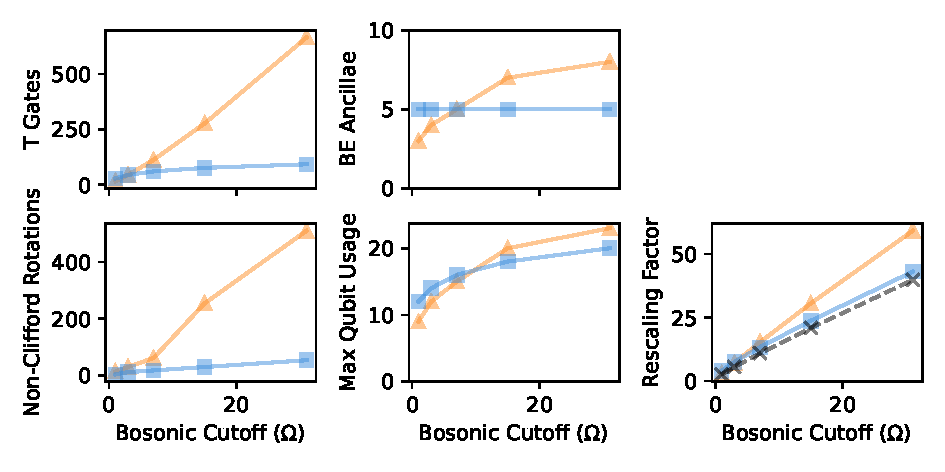
\includegraphics[width = 15cm]{figures/static_yukawa.pdf}
    \caption{Costs associated with a single block encoding of the static Yukawa Hamiltonian \ref{eq:static-yukawa} for LOBE (blue) and LCU (orange).}
    \label{fig:static_yukawa}
\end{figure}